%!TEX root = ../../Compte-rendu.tex

\begin{figure}[H]
	\begin{center}
		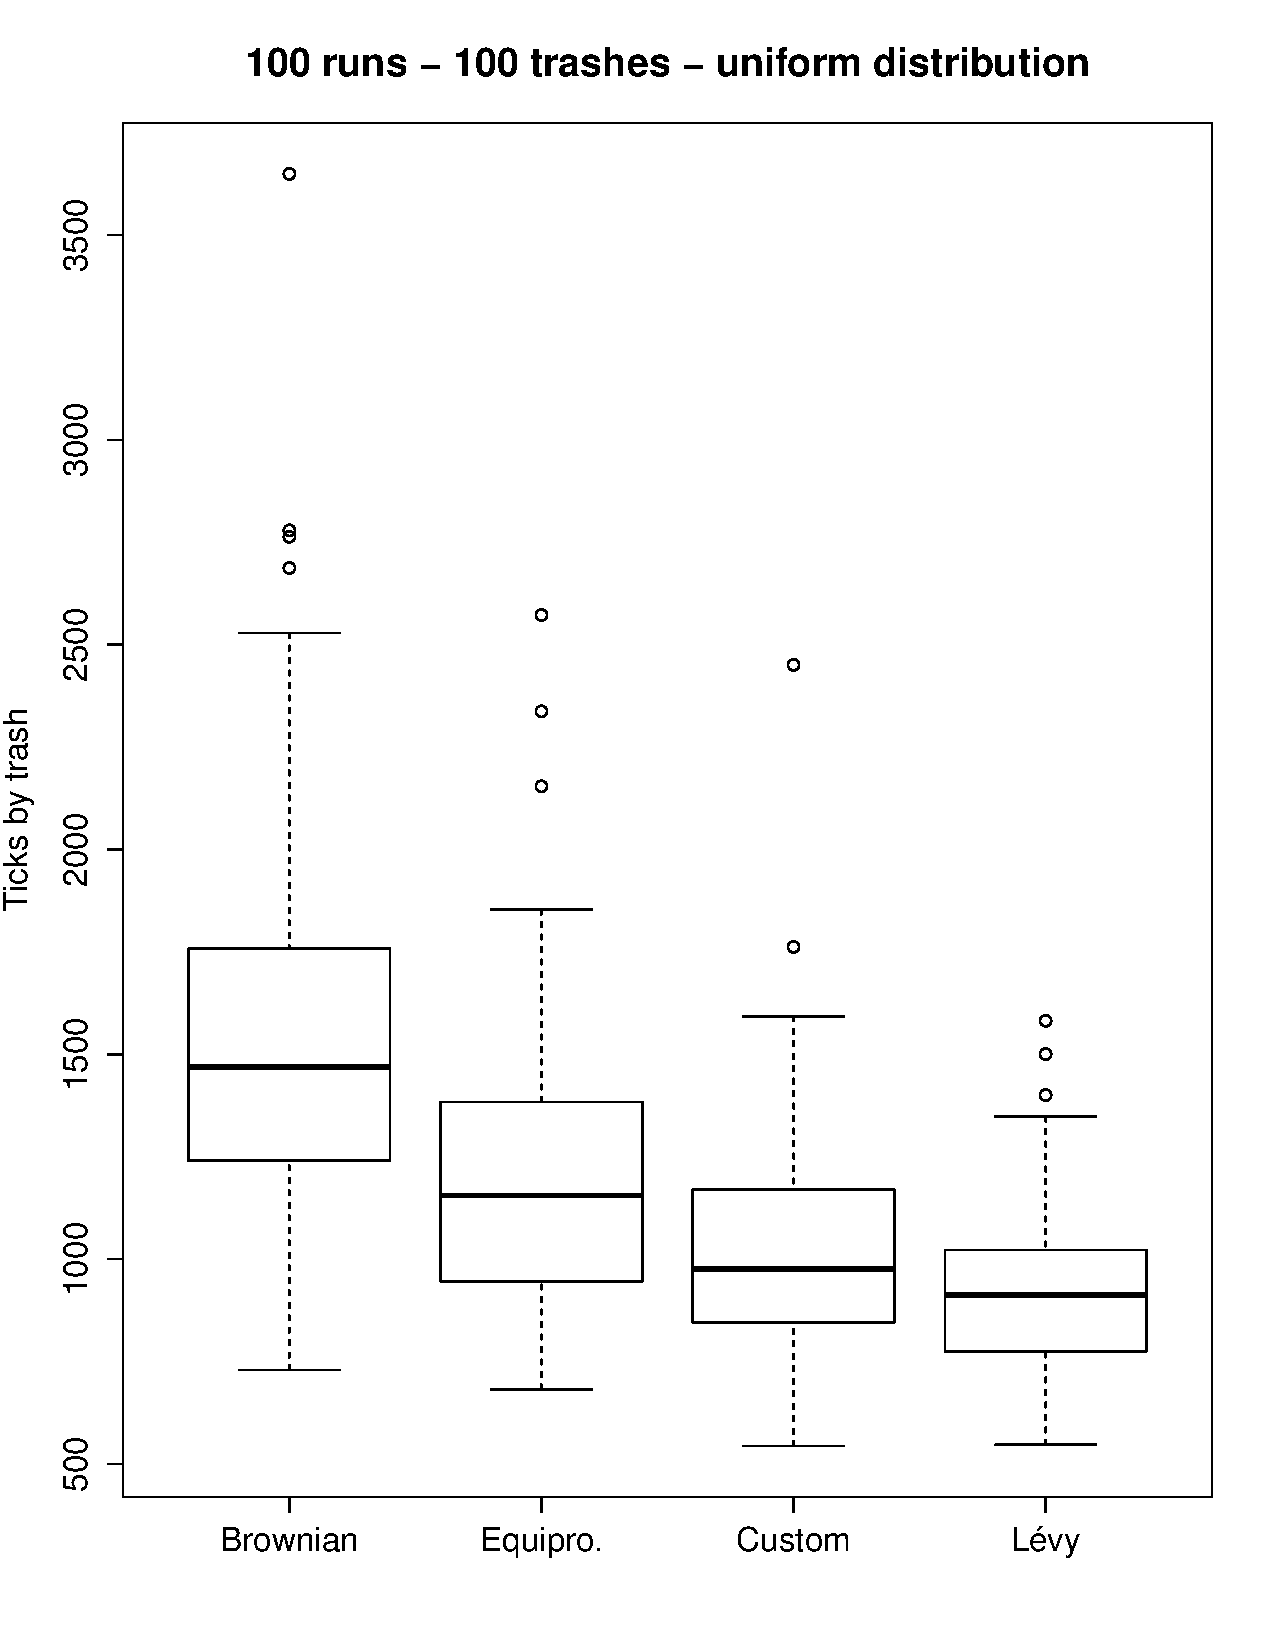
\includegraphics[height=8cm]{diagrams/100TrRnd_all.pdf}
		\caption{}
		\label{fig:100Trashes_Rnd}
	\end{center}
\end{figure}

Nous avons pour les différentes stratégies les médianes suivantes :

\begin{figure}[H]
	\begin{center}
		\begin{tabular}{ | c | c | }
			\hline
			\multicolumn{2}{ | c | }{Médianes pour 100 débris distribués uniformément} \\
			\hline
			Brownian & 1468.673 \\
			Equiprobable & 1155.213 \\
			Custom & 974.9208 \\
			Lévy & 911.797 \\
			\hline
		\end{tabular}
	\end{center}
\end{figure}

En partant de la stratégie Brownian et en allant à celle de Lévy
en passant par Equiprobable et Custom, nous pouvons constater
que nous avons de meilleurs résultats, que ce soit pour leur médiane
comme pour leur fiabilité ainsi que leur valeur minimale et maximale.
